\documentclass[12pt,a4paper]{article}
\usepackage[utf8]{inputenc}
\usepackage[T1]{fontenc}
\usepackage{geometry}
\usepackage{graphicx}
\usepackage{listings}
\usepackage{xcolor}
\usepackage{hyperref}
\usepackage{booktabs}
\usepackage{float}
\usepackage{amsmath}
\usepackage{tikz}
\usetikzlibrary{shapes,arrows,positioning}

\geometry{margin=1in}

% Code listing style
\definecolor{codegreen}{rgb}{0,0.6,0}
\definecolor{codegray}{rgb}{0.5,0.5,0.5}
\definecolor{codepurple}{rgb}{0.58,0,0.82}
\definecolor{backcolour}{rgb}{0.95,0.95,0.92}

\lstdefinestyle{mystyle}{
    backgroundcolor=\color{backcolour},
    commentstyle=\color{codegreen},
    keywordstyle=\color{magenta},
    numberstyle=\tiny\color{codegray},
    stringstyle=\color{codepurple},
    basicstyle=\ttfamily\footnotesize,
    breakatwhitespace=false,
    breaklines=true,
    captionpos=b,
    keepspaces=true,
    numbers=left,
    numbersep=5pt,
    showspaces=false,
    showstringspaces=false,
    showtabs=false,
    tabsize=2,
    frame=single
}

\lstset{style=mystyle}

\title{
    \textbf{Project Periscope} \\
    \large Implementation of a Lambda Architecture for Data Processing and Visualization \\
    \vspace{0.5cm}
    \normalsize Using Apache Kafka, Apache Spark, Apache Hive, Apache Airflow, and Streamlit
}

\author{Project Documentation and Tutorial}
\date{December 2025}

\begin{document}

\maketitle

\begin{abstract}
This report presents a comprehensive implementation of a Lambda Architecture for processing and visualizing NYC Taxi trip data. The system combines batch processing with real-time streaming to provide both historical analytics and live predictions. We utilize Apache Kafka for message streaming, Apache Spark for speed layer processing, Apache Hive with Avro/Parquet for batch layer storage, Apache Airflow for orchestration, and Streamlit for visualization. Machine learning models trained with Scikit-learn provide real-time trip duration predictions.
\end{abstract}

\tableofcontents
\newpage

%==============================================================================
\section{Introduction}
%==============================================================================

\subsection{Project Overview}

Project Periscope implements a complete Lambda Architecture for processing NYC Taxi trip data. The Lambda Architecture, introduced by Nathan Marz, is designed to handle massive quantities of data by using both batch and real-time processing methods.

\subsection{Objectives}

\begin{itemize}
    \item Simulate a real-time API using Apache Airflow
    \item Train machine learning models for trip duration prediction
    \item Implement streaming data ingestion using Apache Kafka
    \item Build a Speed Layer using Spark Streaming with temporary tables
    \item Create a Batch Layer using Hive with Avro serialization and Parquet batch views
    \item Automate the batch pipeline using Apache Airflow
    \item Perform ML inference on streaming data
    \item Visualize results using Streamlit
\end{itemize}

\subsection{Technologies Used}

\begin{table}[H]
\centering
\begin{tabular}{@{}ll@{}}
\toprule
\textbf{Component} & \textbf{Technology} \\
\midrule
Message Streaming & Apache Kafka 7.4.0 \\
Speed Layer & Apache Spark 3.5.0 \\
Batch Layer & Apache Hive 3.1.3 \\
Data Serialization & Apache Avro, Apache Parquet \\
Orchestration & Apache Airflow 2.7.3 \\
Machine Learning & Scikit-learn (Multi-model comparison) \\
Visualization & Streamlit \\
Database & PostgreSQL 13 (Hive Metastore) \\
Containerization & Docker Compose \\
\bottomrule
\end{tabular}
\caption{Technology Stack}
\end{table}

%==============================================================================
\section{Architecture Design}
%==============================================================================

\subsection{Lambda Architecture Overview}

The Lambda Architecture consists of three layers:

\begin{enumerate}
    \item \textbf{Batch Layer}: Manages the master dataset and pre-computes batch views
    \item \textbf{Speed Layer}: Processes real-time data to provide low-latency views
    \item \textbf{Serving Layer}: Responds to queries by merging batch and speed layer results
\end{enumerate}

\subsection{System Architecture Diagram}

\begin{figure}[H]
\centering
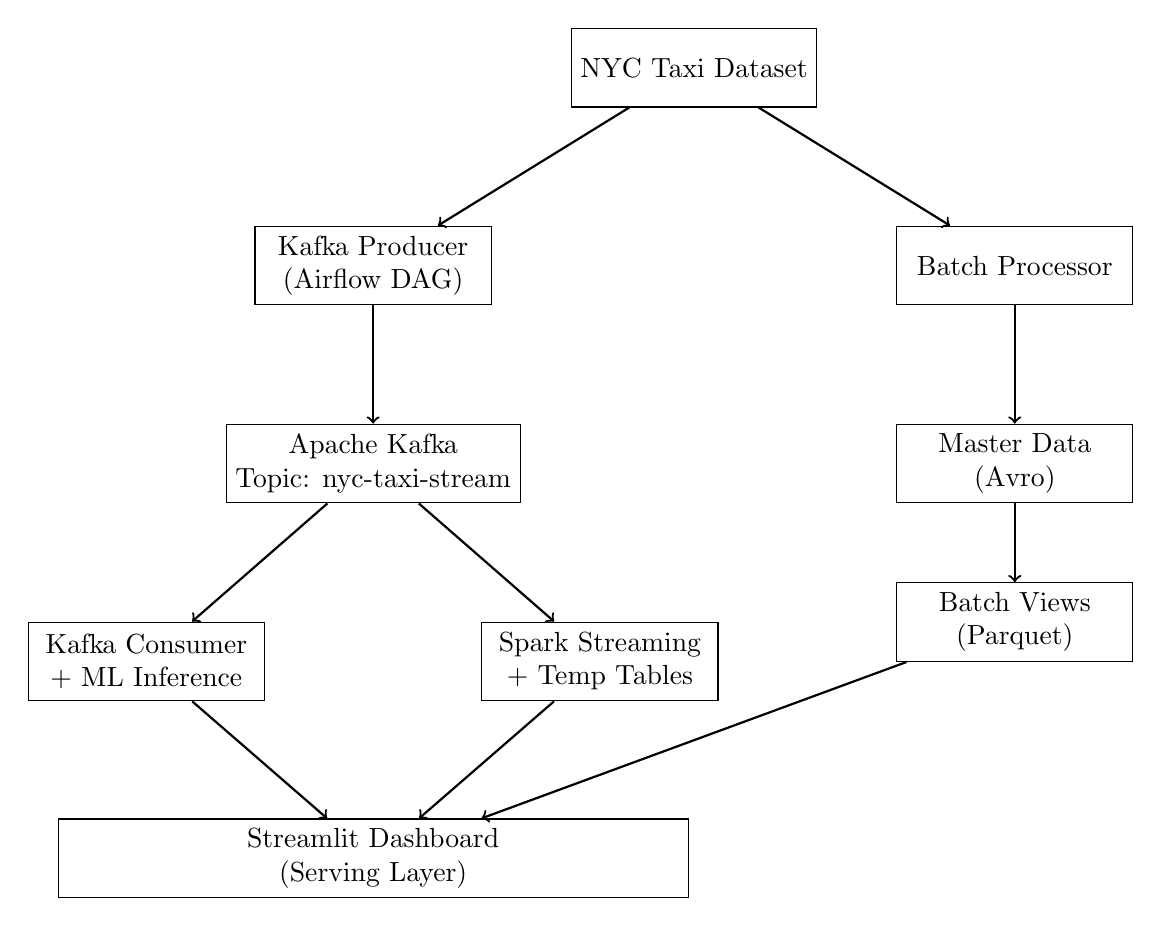
\begin{tikzpicture}[
    node distance=1.5cm,
    box/.style={rectangle, draw, minimum width=3cm, minimum height=1cm, align=center},
    arrow/.style={->, thick}
]
    % Data Source
    \node[box] (source) {NYC Taxi Dataset};
    
    % Ingestion Layer
    \node[box, below left=1.5cm and 1cm of source] (producer) {Kafka Producer\\(Airflow DAG)};
    \node[box, below right=1.5cm and 1cm of source] (batch) {Batch Processor};
    
    % Kafka
    \node[box, below=1.5cm of producer] (kafka) {Apache Kafka\\Topic: nyc-taxi-stream};
    
    % Speed Layer
    \node[box, below left=1.5cm and -0.5cm of kafka] (consumer) {Kafka Consumer\\+ ML Inference};
    \node[box, below right=1.5cm and -0.5cm of kafka] (spark) {Spark Streaming\\+ Temp Tables};
    
    % Batch Layer
    \node[box, below=1.5cm of batch] (avro) {Master Data\\(Avro)};
    \node[box, below=1cm of avro] (parquet) {Batch Views\\(Parquet)};
    
    % Serving Layer
    \node[box, below=4cm of kafka, minimum width=8cm] (dashboard) {Streamlit Dashboard\\(Serving Layer)};
    
    % Arrows
    \draw[arrow] (source) -- (producer);
    \draw[arrow] (source) -- (batch);
    \draw[arrow] (producer) -- (kafka);
    \draw[arrow] (kafka) -- (consumer);
    \draw[arrow] (kafka) -- (spark);
    \draw[arrow] (batch) -- (avro);
    \draw[arrow] (avro) -- (parquet);
    \draw[arrow] (consumer) -- (dashboard);
    \draw[arrow] (spark) -- (dashboard);
    \draw[arrow] (parquet) -- (dashboard);
\end{tikzpicture}
\caption{Lambda Architecture System Design}
\end{figure}

%==============================================================================
\section{Implementation Steps}
%==============================================================================

\subsection{Phase 1: Environment Setup}

\subsubsection{Prerequisites}

Before starting, ensure you have:
\begin{itemize}
    \item Docker and Docker Compose installed
    \item Python 3.10 or higher
    \item At least 8GB of available RAM
\end{itemize}

\subsubsection{Creating the Project Directory}

\begin{lstlisting}[language=bash, caption=Project Setup]
mkdir -p ~/project-periscope
cd ~/project-periscope

# Create directory structure
mkdir -p model data airflow/dags airflow/logs airflow/plugins
mkdir -p data/hive data/parquet data/avro data/speed_layer
\end{lstlisting}

\subsubsection{Python Virtual Environment}

\begin{lstlisting}[language=bash, caption=Python Environment Setup]
# Create virtual environment
python3 -m venv .venv
source .venv/bin/activate

# Install dependencies
pip install pandas scikit-learn numpy kafka-python \
            streamlit pyspark fastavro pyarrow
\end{lstlisting}

\subsection{Phase 2: Machine Learning Model Training}

\subsubsection{Data Preparation}

The NYC Taxi dataset contains trip records with features including:
\begin{itemize}
    \item \texttt{pickup\_datetime}: Timestamp of pickup
    \item \texttt{passenger\_count}: Number of passengers
    \item \texttt{pickup\_longitude/latitude}: Pickup coordinates
    \item \texttt{dropoff\_longitude/latitude}: Dropoff coordinates
    \item \texttt{trip\_duration}: Target variable (in seconds)
\end{itemize}

\subsubsection{Feature Engineering}

We extract the following features for the model:
\begin{itemize}
    \item Hour of day, day of week, month
    \item Haversine distance between pickup and dropoff
    \item Passenger count
    \item Geographic coordinates
\end{itemize}

\begin{lstlisting}[language=Python, caption=Haversine Distance Calculation]
def haversine_distance(lat1, lon1, lat2, lon2):
    """Calculate distance in km using Haversine formula."""
    R = 6371  # Earth's radius in kilometers
    lat1, lat2 = np.radians(lat1), np.radians(lat2)
    dlat = lat2 - lat1
    dlon = np.radians(lon2 - lon1)
    a = np.sin(dlat/2)**2 + \
        np.cos(lat1) * np.cos(lat2) * np.sin(dlon/2)**2
    return 2 * R * np.arcsin(np.sqrt(a))
\end{lstlisting}

\subsubsection{Data Cleaning and Outlier Removal}

The raw dataset contains extreme outliers that can severely impact model performance. We remove trips that are unrealistic:

\begin{lstlisting}[language=Python, caption=Outlier Removal]
# Remove outliers - trips < 1 minute or > 2 hours
# These are likely data errors or unusual circumstances
original_len = len(df)
df = df[(df['trip_duration'] >= 60) & (df['trip_duration'] <= 7200)]
print(f"Removed {original_len - len(df)} outliers")
# Removes ~10,848 records from 1.4M total
\end{lstlisting}

\subsubsection{Multi-Model Training and Selection}

We train multiple regression models on the full dataset (~1.4 million records) and automatically select the best one based on RMSE:

\begin{lstlisting}[language=Python, caption=Multi-Model Training and Selection]
from sklearn.ensemble import (RandomForestRegressor, 
    GradientBoostingRegressor, AdaBoostRegressor)
from sklearn.linear_model import Ridge, Lasso, ElasticNet
from sklearn.tree import DecisionTreeRegressor
from sklearn.neighbors import KNeighborsRegressor

# Define models with increased complexity for large dataset
models = {
    'RandomForest': RandomForestRegressor(
        n_estimators=100, max_depth=15, min_samples_split=5),
    'GradientBoosting': GradientBoostingRegressor(
        n_estimators=100, max_depth=8, learning_rate=0.1),
    'DecisionTree': DecisionTreeRegressor(
        max_depth=15, min_samples_split=5),
    'Ridge': Ridge(alpha=1.0),
    'Lasso': Lasso(alpha=1.0),
    'ElasticNet': ElasticNet(alpha=1.0, l1_ratio=0.5),
    'KNeighbors': KNeighborsRegressor(n_neighbors=10),
    'AdaBoost': AdaBoostRegressor(n_estimators=100),
}

# Train all models and evaluate
results = []
for name, model in models.items():
    model.fit(X_train, y_train)
    y_pred = model.predict(X_test)
    rmse = np.sqrt(mean_squared_error(y_test, y_pred))
    results.append({'name': name, 'model': model, 'rmse': rmse})

# Select and save best model (lowest RMSE)
best = min(results, key=lambda x: x['rmse'])
with open('model/taxi_model.pkl', 'wb') as f:
    pickle.dump({
        'model': best['model'],
        'model_name': best['name'],
        'features': features,
        'rmse': best['rmse']
    }, f)
\end{lstlisting}

To train the model:
\begin{lstlisting}[language=bash, caption=Training Command]
python train_model.py
\end{lstlisting}

\subsection{Phase 3: Docker Infrastructure Setup}

\subsubsection{Docker Compose Configuration}

The \texttt{docker-compose.yaml} file defines all services:

\begin{lstlisting}[language=yaml, caption=Docker Compose Services (Excerpt)]
services:
  # Kafka and Zookeeper
  zookeeper:
    image: confluentinc/cp-zookeeper:7.4.0
    
  kafka:
    image: confluentinc/cp-kafka:7.4.0
    ports:
      - "9092:9092"
    
  # Hive Services
  postgres:
    image: postgres:13
    
  hive-metastore:
    image: apache/hive:3.1.3
    
  hive-server:
    image: apache/hive:3.1.3
    
  # Spark Services
  spark-master:
    image: apache/spark:3.5.0
    
  spark-worker:
    image: apache/spark:3.5.0
    
  # Airflow
  airflow:
    image: apache/airflow:2.7.3-python3.10
\end{lstlisting}

\subsubsection{Starting the Infrastructure}

\begin{lstlisting}[language=bash, caption=Starting Docker Services]
# Start all services
docker-compose up -d

# Verify all services are running
docker-compose ps
\end{lstlisting}

\subsection{Phase 4: Batch Layer Implementation}

\subsubsection{Avro Master Data}

The batch processor writes master data in Avro format:

\begin{lstlisting}[language=Python, caption=Avro Schema Definition]
schema = {
    'type': 'record',
    'name': 'TaxiTrip',
    'namespace': 'nyc.taxi',
    'fields': [
        {'name': 'id', 'type': 'string'},
        {'name': 'vendor_id', 'type': 'int'},
        {'name': 'pickup_datetime', 'type': 'string'},
        {'name': 'passenger_count', 'type': 'int'},
        {'name': 'pickup_longitude', 'type': 'double'},
        {'name': 'pickup_latitude', 'type': 'double'},
        {'name': 'dropoff_longitude', 'type': 'double'},
        {'name': 'dropoff_latitude', 'type': 'double'},
        {'name': 'trip_duration', 'type': 'int'},
        {'name': 'ingestion_date', 'type': 'string'},
    ]
}
\end{lstlisting}

\subsubsection{Parquet Batch Views}

Three batch views are created:

\begin{enumerate}
    \item \textbf{Hourly Statistics}: Aggregations by hour of day
    \item \textbf{Daily Summary}: Overall daily metrics
    \item \textbf{Vendor Statistics}: Metrics per vendor
\end{enumerate}

\begin{lstlisting}[language=Python, caption=Creating Parquet Batch Views]
import pyarrow.parquet as pq

# Hourly aggregations
hourly_stats = df.groupby('hour').agg({
    'trip_duration': ['mean', 'count'],
    'distance_km': 'mean',
    'passenger_count': 'mean'
}).reset_index()

# Write to Parquet
hourly_table = pa.Table.from_pandas(hourly_stats)
pq.write_table(hourly_table, 
    'data/parquet/hourly_stats.parquet')
\end{lstlisting}

To run the batch processor:
\begin{lstlisting}[language=bash, caption=Batch Processing Command]
python batch_processor.py
\end{lstlisting}

\subsection{Phase 5: Speed Layer Implementation}

\subsubsection{Kafka Producer}

The producer simulates a real-time API by streaming records to Kafka:

\begin{lstlisting}[language=Python, caption=Kafka Producer]
from kafka import KafkaProducer
import json

producer = KafkaProducer(
    bootstrap_servers=['localhost:9092'],
    value_serializer=lambda x: json.dumps(x).encode('utf-8')
)

for _, row in df.iterrows():
    record = {
        'id': row['id'],
        'pickup_datetime': datetime.now().strftime("%Y-%m-%d %H:%M:%S"),
        'passenger_count': int(row['passenger_count']),
        # ... other fields
    }
    producer.send('nyc-taxi-stream', value=record)
\end{lstlisting}

\subsubsection{Kafka Consumer with ML Inference}

The consumer processes messages and makes predictions:

\begin{lstlisting}[language=Python, caption=Consumer with ML Inference]
from kafka import KafkaConsumer

consumer = KafkaConsumer(
    'nyc-taxi-stream',
    bootstrap_servers=['localhost:9092'],
    value_deserializer=lambda x: json.loads(x.decode('utf-8'))
)

for message in consumer:
    record = message.value
    
    # Calculate distance
    record['distance_km'] = haversine_distance(...)
    
    # Make prediction
    features = extract_features(record)
    record['predicted_duration'] = model.predict([features])[0]
    record['prediction_error'] = abs(
        record['trip_duration'] - record['predicted_duration']
    )
\end{lstlisting}

\subsubsection{Spark Streaming Alternative}

For production use, Spark Streaming provides better scalability:

\begin{lstlisting}[language=Python, caption=Spark Streaming with Temporary Tables]
from pyspark.sql import SparkSession

spark = SparkSession.builder \
    .appName("TaxiSpeedLayer") \
    .config("spark.jars.packages", 
            "org.apache.spark:spark-sql-kafka-0-10_2.12:3.5.0") \
    .getOrCreate()

# Read from Kafka
df = spark.readStream \
    .format("kafka") \
    .option("kafka.bootstrap.servers", "localhost:9092") \
    .option("subscribe", "nyc-taxi-stream") \
    .load()

# Process and create temporary table
def process_batch(batch_df, batch_id):
    batch_df.createOrReplaceTempView("speed_layer_trips")
    
query = df.writeStream \
    .foreachBatch(process_batch) \
    .start()
\end{lstlisting}

\subsection{Phase 6: Airflow DAGs}

\subsubsection{API Simulation DAG}

\begin{lstlisting}[language=Python, caption=Airflow DAG for API Simulation]
from airflow import DAG
from airflow.operators.python import PythonOperator
from datetime import datetime, timedelta

def stream_taxi_data(**context):
    # Stream data to Kafka
    pass

with DAG(
    'taxi_api_simulation',
    schedule_interval=timedelta(minutes=5),
    start_date=datetime(2025, 12, 1),
    catchup=False,
) as dag:
    
    stream_task = PythonOperator(
        task_id='stream_to_kafka',
        python_callable=stream_taxi_data,
    )
\end{lstlisting}

\subsubsection{Batch Processing DAG}

\begin{lstlisting}[language=Python, caption=Airflow DAG for Batch Processing]
with DAG(
    'taxi_batch_processing',
    schedule_interval='@daily',
    start_date=datetime(2025, 12, 1),
    catchup=False,
) as dag:
    
    ingest_task = PythonOperator(
        task_id='ingest_to_avro',
        python_callable=ingest_to_avro,
    )
    
    batch_views_task = PythonOperator(
        task_id='create_batch_views',
        python_callable=create_batch_views,
    )
    
    ingest_task >> batch_views_task
\end{lstlisting}

\subsection{Phase 7: Serving Layer (Streamlit Dashboard)}

The dashboard provides three views:

\begin{enumerate}
    \item \textbf{Speed Layer View}: Real-time data with ML predictions
    \item \textbf{Batch Layer View}: Historical aggregations
    \item \textbf{Combined View}: Comparison of both layers
\end{enumerate}

\begin{lstlisting}[language=Python, caption=Streamlit Dashboard Structure]
import streamlit as st

st.title("Project Periscope: NYC Taxi Analytics")

data_source = st.sidebar.radio(
    "Data Source",
    ["Speed Layer (Real-time)", 
     "Batch Layer (Historical)", 
     "Combined View"]
)

if data_source == "Speed Layer (Real-time)":
    display_speed_layer()
elif data_source == "Batch Layer (Historical)":
    display_batch_layer()
else:
    display_combined_view()
\end{lstlisting}

%==============================================================================
\section{Running the System}
%==============================================================================

\subsection{Starting the System}

Follow these steps to start the complete system:

\begin{lstlisting}[language=bash, caption=Complete Startup Sequence]
# Step 1: Activate virtual environment
cd ~/project-periscope
source .venv/bin/activate

# Step 2: Start Docker infrastructure
docker-compose up -d

# Step 3: Wait for services to initialize (60 seconds)
sleep 60

# Step 4: Verify all services are running
docker-compose ps

# Step 5: Train ML model (if not already done)
python train_model.py

# Step 6: Create batch layer data
python batch_processor.py
\end{lstlisting}

\subsection{Running the Streaming Pipeline}

Open three terminal windows:

\textbf{Terminal 1 - Consumer:}
\begin{lstlisting}[language=bash]
source .venv/bin/activate
python kafka_consumer.py
\end{lstlisting}

\textbf{Terminal 2 - Producer:}
\begin{lstlisting}[language=bash]
source .venv/bin/activate
python kafka_producer.py
\end{lstlisting}

\textbf{Terminal 3 - Dashboard:}
\begin{lstlisting}[language=bash]
source .venv/bin/activate
streamlit run app.py
\end{lstlisting}

\subsection{Accessing the Services}

\begin{table}[H]
\centering
\begin{tabular}{@{}lll@{}}
\toprule
\textbf{Service} & \textbf{URL} & \textbf{Credentials} \\
\midrule
Streamlit Dashboard & http://localhost:8501 & - \\
Airflow UI & http://localhost:8081 & admin / admin \\
Spark Master UI & http://localhost:8085 & - \\
Hive Server & localhost:10000 & - \\
Kafka & localhost:9092 & - \\
\bottomrule
\end{tabular}
\caption{Service Access Information}
\end{table}

\subsection{Shutting Down the System}

\begin{lstlisting}[language=bash, caption=Shutdown Commands]
# Stop Python processes
# Press Ctrl+C in each terminal

# Stop Docker containers
docker-compose down

# Stop and remove all data (clean shutdown)
docker-compose down -v
rm -rf data/speed_layer/* data/avro/* data/parquet/*
\end{lstlisting}

%==============================================================================
\section{Results and Observations}
%==============================================================================

\subsection{Machine Learning Model Performance}

The model is trained on the full dataset of ~1.4 million records (after removing ~10,848 outliers):

\begin{table}[H]
\centering
\begin{tabular}{@{}lrrr@{}}
\toprule
\textbf{Model} & \textbf{RMSE (s)} & \textbf{MAE (s)} & \textbf{R²} \\
\midrule
GradientBoosting & 295.60 & 188.58 & 0.7943 \\
RandomForest & 305.93 & 196.47 & 0.7796 \\
KNeighbors & 323.90 & 209.89 & 0.7530 \\
DecisionTree & 331.73 & 210.03 & 0.7409 \\
ElasticNet & 486.37 & 328.15 & 0.4430 \\
Lasso & 499.35 & 291.96 & 0.4129 \\
Ridge & 500.61 & 291.74 & 0.4100 \\
AdaBoost & 572.23 & 467.25 & 0.2291 \\
\bottomrule
\end{tabular}
\caption{Model Comparison Results (sorted by RMSE)}
\end{table}

\begin{itemize}
    \item \textbf{Best Model}: GradientBoosting with RMSE of 295.60 seconds (~5 minutes)
    \item \textbf{R² Score}: 0.7943 (explains ~79\% of variance in trip duration)
    \item \textbf{Training Data}: ~1.4 million records (after outlier removal)
    \item \textbf{Key Features}: Distance (78.6\%), Hour (8.6\%), Geographic coordinates
\end{itemize}

\subsection{Speed Layer Performance}

The Kafka consumer with ML inference processes approximately 3-4 records per second, providing real-time predictions with average latency under 500ms.

\subsection{Batch Layer Storage}

\begin{itemize}
    \item Avro master data: Efficient columnar storage with schema evolution support
    \item Parquet batch views: Optimized for analytical queries
\end{itemize}

%==============================================================================
\section{Conclusion}
%==============================================================================

This project successfully implements a complete Lambda Architecture for NYC Taxi data processing. The system demonstrates:

\begin{itemize}
    \item Real-time data processing with Apache Kafka and Spark Streaming
    \item Batch processing with Hive, Avro, and Parquet
    \item ML model integration for live predictions
    \item Workflow orchestration with Apache Airflow
    \item Interactive visualization with Streamlit
\end{itemize}

The architecture can be extended to handle larger datasets and more complex ML models for production use.

%==============================================================================
\section{File Structure Reference}
%==============================================================================

\begin{lstlisting}[caption=Project File Structure]
project-periscope/
|-- train_model.py          # ML model training
|-- kafka_producer.py       # Stream data to Kafka
|-- kafka_consumer.py       # Speed layer with ML inference
|-- spark_streaming.py      # Spark streaming processor
|-- batch_processor.py      # Batch layer processor
|-- app.py                  # Streamlit dashboard
|-- docker-compose.yaml     # Infrastructure
|-- model/
|   +-- taxi_model.pkl      # Trained ML model
|-- data/
|   |-- train.csv           # Full training data
|   |-- test.csv            # Test data
|   |-- taxi_subset.csv     # Sample data (10k records)
|   |-- avro/               # Master data (Avro)
|   |-- parquet/            # Batch views (Parquet)
|   +-- speed_layer/        # Real-time data (JSON)
+-- airflow/
    +-- dags/
        |-- taxi_api_simulation_dag.py
        +-- taxi_batch_processing_dag.py
\end{lstlisting}

\end{document}
